\chapter{Introduction}
\label{sec:intro}

% Add Fancy Headers to future pages
\pagestyle{fancy}
%\renewcommand{\sectionmark}[1]{\markright{#1}}
\renewcommand{\sectionmark}[1]{\markright{\thesection\quad \ #1}}
\fancyhead{}
%%%%%%%%%%%%%%%%%%%%%%%%%%%% The paper headers
\fancyhead[LE,RO]{\thepage}
\fancyhead[LO]{\text{Chapter 1} \quad   {Introduction}}
\fancyhead[RE]{\sectionmark \quad \rightmark } %Even page header and number at left top
\fancyfoot[L,R,C]{}
\renewcommand{\headrulewidth}{1pt}% disable the underline of the header part

The theory of waves and wave propagation in periodic media has influenced many fields in the physical sciences, dating back to the influential work of Lord Rayleigh. The advancement of information and communication technologies was made possible by the use of various manifestations of waves, most notably electromagnetic waves to transmit information around the world and electrons to process information in computers. The role of wave phenomena will continue to grow in the future, especially in emerging fields of science and technology such as cryptography, medical imaging, and quantum computing. Because of the increased availability of parallel processing and high-performance computing, computer simulation has become an essential component of wave simulation, supplementing both theory and experiment. As a result, this thesis aims to extend a class of fast and robust numerical methods (known as HOPS) to simulate certain wave phenomena in a regime that is characterized by a periodic structure.

The remainder of this introductory chapter will give a brief history of the field of wave scattering and discuss early achievements of scientists and practitioners. The mathematical notation used in later sections will be introduced alongside the geometry of a two--layer periodic structure. We will also introduce the Rayleigh expansions, electromagnetic waves, TE polarization, TM polarization, and discuss the motivation behind our \gls{hops} schemes.

\section{History}
\label{intro:history}
The scattering of acoustic and electromagnetic waves by rough interfaces has been the subject of considerable study for more than a century \cite{varadan2013low}. Lord Rayleigh first investigated this problem in 1881 \cite{rayleigh1881x} and provided the foundation on which almost all subsequent work is based. It is possible to gain a good understanding of the mechanics of this field of scientific study and its application in light scattering by reading the works of van de Hülst (1957) \cite{hulst1981light}, Twersky (1964) \cite{twersky1964rayleigh}, Kerker (1969) \cite{Kerker1969TheSO}, Petit (1980) \cite{Petit80}, and Wilcox (1984) \cite{Wilcox84}. For the interested reader, we recommend the Habilitationsschrift of T. Arens (2009) \cite{ArensHab} as a definitive reference for periodic layered media problems and for the the state-of-the-art analysis of solutions to the Helmholtz and Maxwell equations in two and three dimensions.

Scattering is a process that alters the direction of light and is commonly associated with light's interaction with small particles \cite{choudhury2014principles}. Light scatters and travels in many directions other than the propagating direction as a result of this. Light is scattered by reflection and refraction in relatively large particles, such as pigments with dimensions greater than 2.0 $\mu$m. Diffraction occurs when light is scattered by relatively small particles with dimensions less than about 0.3 $\mu$m. When the sun is high in the sky during the day, the sky appears blue because blue light is scattered more effectively by very small particles in the atmosphere than light of longer wavelengths. When the sun is low on the horizon at sunrise and sunset, we see more of the non-scattered light, and the sky appears red. 

The majority of the objects we see are visible due to light scattering from their surfaces.  This is, after all, our fundamental physical observation method \cite{Kerker1969TheSO}. Light scattering is determined by the wavelength or frequency of the light being scattered. Because visible light has a wavelength on the order of a micron, objects much smaller than this cannot be seen, even with a microscope. Lord Rayleigh was among the first to explain light scattering by very
small particles. Rayleigh's observations show that the intensity of light scattered varies \cite{choudhury2014principles}:
\begin{itemize}
    \item Directly based on the intensity of incident light.
    \item Directly based on the average volume of scattering particles.
\end{itemize}
Lord Rayleigh also discovered that light can scatter without the use of scattering particles. This is due to the fact that changes in refractive index at different parts of a material can be sufficient to cause scattering. If a material is homogeneous, then the composition of all infinitesimal volume elements is the same and optical properties which define the material response to the incident radiation, such as transmissivity, reflectivity, and absorptivity are also the same. The aforementioned properties vary in different directions in a heterogeneous material, resulting in light scattering. On a macroscopic scale, optical properties vary over distances less than the wavelength of the incident light, resulting in the scattering of energy away from the direction of propagation. 

The result of Rayleigh's observations that scattering depends on the wavelength and, thus, the color of the light is  now known as the Rayleigh scattering law \cite{rayleigh1871scattering,lord1871light}. To answer the question: ``Why is the sky blue in the afternoon and red at sunset or sunrise?" one may observe that blue light has a wavelength of around 400 nanometers, while red light has a wavelength of about 700 nanometers. The scattering law states that the percentage of light that will be scattered is inversely proportional to the fourth power of the wavelength. Therefore, blue light, which is at the short wavelength end of the visible spectrum, will be scattered much more strongly than red light, which is at the long wavelength end of the visible spectrum. The white light from the sun scatters and splits into different components due to particles in our environment that are roughly the same size as the wavelength of visible light.
Because of their small size, oxygen and nitrogen (the major components of our atmosphere) scatter violet and blue light.  This results in the blue color of the afternoon sky, since, in directions other than towards the Sun, the observer sees predominantly scattered light. In contrast, the distance that light must travel from the Sun to an observer is highest at sunrise and dusk. This signifies that a substantial proportion of blue and violet light has been scattered, resulting in light that is predominantly of a longer wavelength and appears red to an observer. 
\vspace{-17mm}
\begin{figure}[H]
\centering
    \subfloat[Blue Sky (Afternoon)]
    {{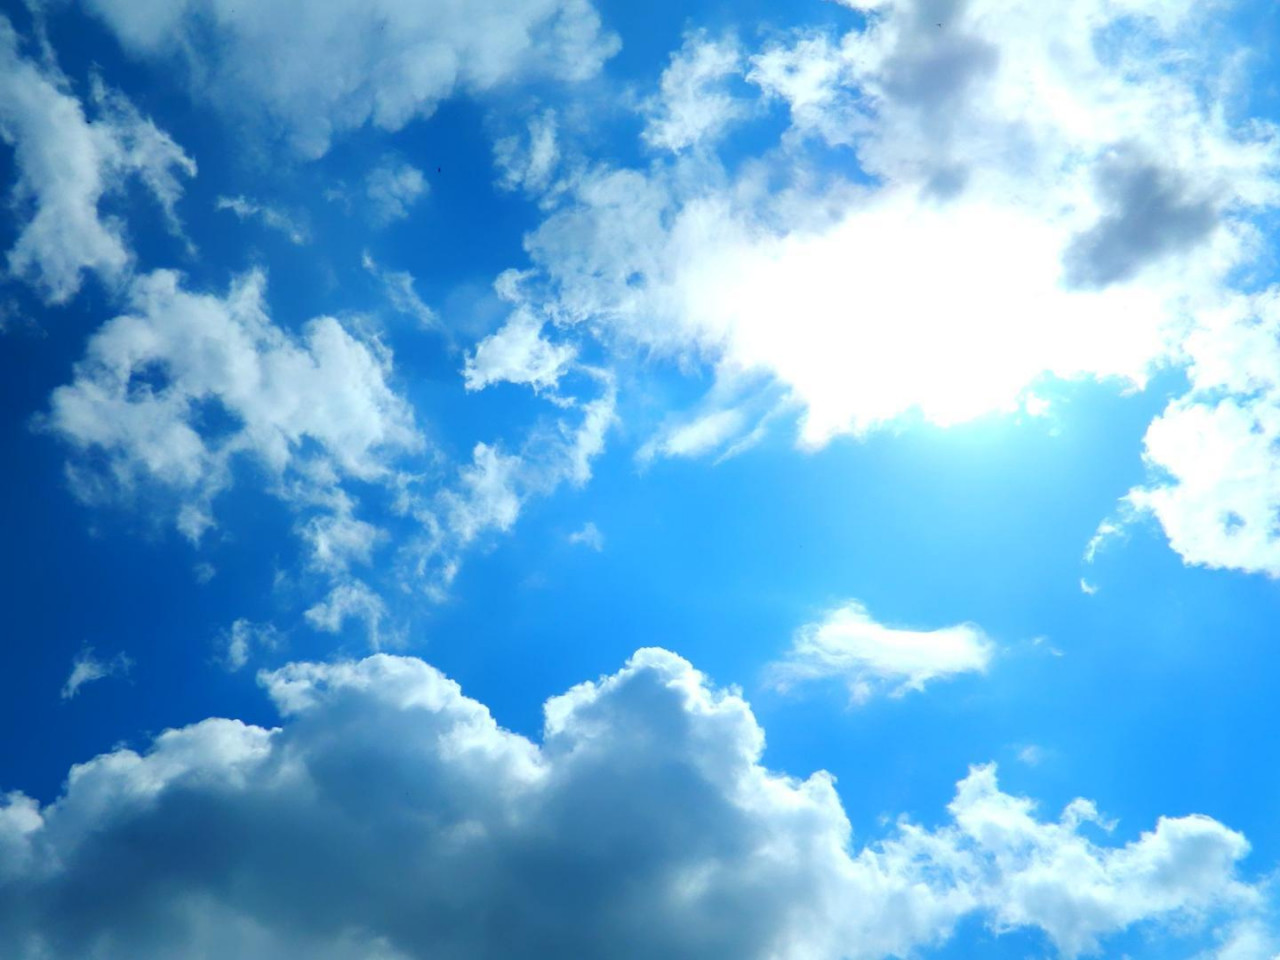
\includegraphics[width=7.15cm]{figures/blue_sky.png} }}
    \subfloat[Red Sky (Dawn and Dusk)]
    {{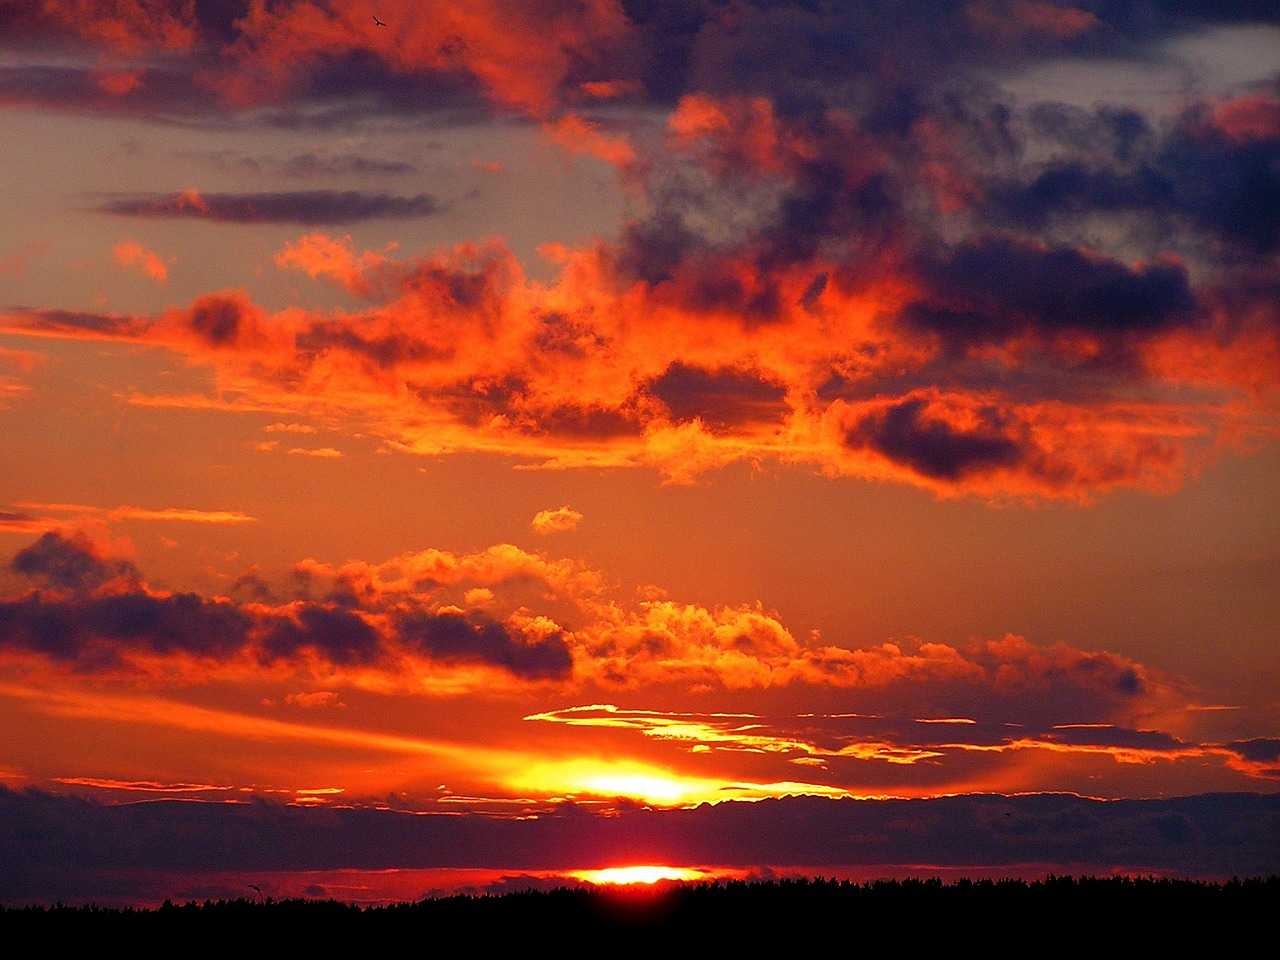
\includegraphics[width=7.15cm]{figures/red_sky.png} }}
%\includegraphics[width=0.5\textwidth]{conv_N}
\vspace{3mm}
\caption{Rayleigh scattering is responsible for the sky's blue tint during the day and the Sun's reddening at sunset and sunrise.}
%\label{Fig:N}
\end{figure}
\vspace{-18mm}
Research in the twentieth century focused on the subject of scattering from particles. In this, numerous authors contributed to the general theory of scattering by acoustic and electromagnetic waves. L. Foldy was among the first to present a complete framework \cite{foldy1945multiple} for the multiple scattering of a random distribution of particles. He considered the multiple scattering of scalar waves by a random distribution of isotropic scatterers through averaging a medium of uncorrelated, isotropic, point scatterers. M. Lax then expanded Foldy's work by including anisotropic scattering and pairwise correlation between particles \cite{lax1951multiple}. V. Twersky later extended this work through investigating the scattering of waves by multiple spheres and cylinders in a fluid, which would later lead to research in the scattering of multiple dense objects \cite{fikioris1964multiple,waterman1961multiple}, grating scattering \cite{twersky1973multiple}, and the propagation of plane--compressible waves in fiber-reinforced composites \cite{varadan1978multiple,sheng2007introduction,tsang2004scattering}. 

In 1952, Twersky published a sequence of manuscripts \cite{twersky1952multiple,twersky1952multipleb,twersky1952multiplec} describing a solution to the problem of multiple scattering of radiation by an arbitrary configuration of parallel cylinders. He developed a formal model in terms of cylindrical wave functions for the scattering of an acoustic or electromagnetic wave by an array of parallel cylindrical structures which takes into account all contributions to the excitation of one cylinder by radiation scattered by the others. He then extended his solution to the case where all axes of the cylinders lie in the same plane \cite{kavakliouglu2012exact}. In addition, Twersky introduced methods based on Green's function \cite{twersky1956scatttering} to describe the relationship between the scattered amplitude of an infinite grating in terms of the scattered amplitude of a single isolated cylinder. In 1961, Twersky found a method of representing the scattering coefficients in terms of elementary functions based on Schl{\"o}milch series \cite{twersky1961elementary}. Since then, numerous studies have been conducted to confirm Twersky's findings and to expand his analysis on cylindrical gratings (including the research on wave propagation by G. Brown in the 1980s \cite{brown1980coherent,brown1981alternate}).

Many other authors have contributed to the study of multiple scattering effects. J. Keller investigated wave propagation in continuous media through use of stochastic linear differential equations \cite{keller1964stochastic} and by including terms up to the third order in a perturbation expansion \cite{de1998stochastic}. U. Frisch then extended this work by developing a theory of multiple scattering of waves by a continuous random medium through perturbation expansions and approximation methods \cite{frisch1965wave}. Frisch applied the Feyman diagram method to identify the scattering interaction between the random surface and the random medium and demonstrated how to obtain the exact solution of a scalar wave equation by the means of functional space integration. P. Waterman and R. Truell created a rule \cite{waterman1961multiple} to relate the scattered wave and exciting field by defining a linear scattering operator $T$ in a homogeneous isotropic medium governed by the Helmholtz equation. The application of Waterman's rule to scattering characteristics of particles is now known as $T$--matrix formalism in the engineering literature. V. Varadan, V. Bringi, and Y. Ma \cite{varadan1979coherent,varadan1984coherent} then considered vector electromagnetic waves in three--dimensions and investigated various shapes and configurations of particles. In terms of quantum mechanical scattering, L. Tsang, J. Kong, and T. Habashy applied the method of coherent
potential  \cite{tsang1980multiple,tsang1982multiple} to the study of multiple scattering of electromagnetic waves by a random distribution of discrete scatterers. They found that the approach of quasicrystalline approximation was particularly effective in treating electromagnetic scattering by discrete scatterers and can accurately calculate the effective propagation constants of the coherent
wave. Further research is being performed by numerous authors in both the applied mathematics and engineering communities.
\section{Motivation}
\label{intro:motivation}

The scattering of linear electromagnetic waves by a layered structure is a
central model in many problems of scientific and engineering interest. Examples arise in areas such as geophysics \cite{VirieuxOperto09,BleibRondenay09}, imaging \cite{NW01}, materials science \cite{Godreche92}, nanoplasmonics \cite{Raether88,Maier07,EnochBonod12}, and oceanography \cite{BL82}. In the case of nanoplasmonics, there are many topics of interest such as extraordinary optical transmission \cite{ELGTW98}, surface enhanced spectroscopy \cite{Moskovits85}, and surface plasmon resonance biosensing \cite{Homola08,ILWJLNNO11} and \cite{LJJOO12,JJJLWO13,RJOM13,NichollsReitichJohnsonOh14}. In all of the physical problems it is necessary to approximate scattering returns in a fast, robust, and highly accurate fashion. This thesis will expand upon a novel HOPS algorithm \cite{Nicholls14b,NichollsTammali15,NichollsOhJohnsonReitich15} designed for the numerical simulation of the layered periodic media (diffraction or scattering) problem.

A variety of classical algorithms have been used for simulation of this problem. However, recent studies have demonstrated \cite{AmbroseNicholls13,Nicholls14b,nicholls2016high,NichollsOhJohnsonReitich15} that volumetric approaches (such as finite difference and finite/spectral element methods) are greatly disadvantaged when dealing with layered media problems because of
the large number of unknowns. Another natural candidate is an interfacial method based upon integral equations (IEs) \cite{ColtonKress13}. There are, however, also difficulties associated with these, as discussed in \cite{AmbroseNicholls13,Nicholls14b,nicholls2016high,NichollsOhJohnsonReitich15}. In the past few years, a number of these have been addressed through various techniques such as (i) the use of sophisticated quadrature rules to deliver high order spectral accuracy, (ii) the design of preconditioned iterative solvers with appropriate acceleration \cite{GreengardRokhlin87}, and (iii) new tactics to avoid periodizing the Green function \cite{BarnettGreengard11,ChoBarnett15,LaiKobayashiBarnett15}. Despite these alternatives (see, e.g., \cite{ReitichTamma04}), there are two properties that make these strategies noncompetitive in our parametrized setting.  These are:
\begin{enumerate}
    \item For configurations parameterized by a real value $\varepsilon$ (in our scheme the height/slope of the interface), an IE solver will return the scattering returns for only one particular value of $\varepsilon$. If this is changed, the solver must be run again.
    \item IE solvers require inverting a dense, nonsymmetric positive definite system of linear equations for every simulation.
\end{enumerate}
In contrast, the HOPS approach \cite{Nicholls14b,nicholls2016high,NichollsOhJohnsonReitich15} can effectively address these concerns. More specifically, in \cite{nicholls2016high,NichollsOhJohnsonReitich15} an alternative known as the \gls{fe} method is proposed which is based on the low-order calculations of Rayleigh \cite{Rayleigh07} and Rice \cite{Rice51}. An expansion to high order was first introduced by Bruno and Reitich \cite{BrunoReitich93a,BrunoReitich93b,BrunoReitich93c} and then was later enhanced and stabilized by Nicholls, Reitich, and Malcolm \cite{NichollsReitich03a,NichollsReitich03b,NichollsReitich07,MalcolmNicholls10}. This latter method is known as the TFE method. The TFE method maintains all of the classical advantages of IE formulations (such as surface formulation and exact enforcement of far--field and quasi--periodic boundary conditions) while effectively addressing the two shortcomings listed above:
\begin{enumerate}
    \item The method is built upon expanding in the boundary parameter $\varepsilon$. Once the Taylor coefficients are known for the scattering quantities, the TFE method can recover all of the returns by summing the Taylor coefficients. It is unnecessary to begin a new summation for every value of $\varepsilon$. 
    \item The scheme is based on a perturbation of the interface which, at every perturbation order, requires the inversion of a single, sparse operator corresponding to the flat-interface solution.
\end{enumerate}
For a single incident wavelength, the TFE method is among the most efficient available in our layered media setting. A generalization of the HOPS approach developed by Bruno and Reitich is known as an \gls{awe}. The AWE methods \cite{PillageRohrer90,KSNZA96,ReddyDeshpandeCockrellBeck98,SloaneLeeLee01,Nicholls16} are built upon an additional expansion in wavelength (frequency) about a base value and will be a major source of analysis in the second half of our thesis. Our aim is to develop a novel interfacial method using a combined HOPS/AWE algorithm that provides a stable numerical scheme and a rigorous convergence result. We will carefully show that our new algorithm is highly accurate, rapid, robust, and is jointly analytic with respect to two smallness assumptions: (i) an interfacial deformation and (ii) a frequency deformation.
\section{Preliminaries and Notation}
\label{intro:preliminaries_notation
}

We consider a $y$--invariant, doubly layered structure
with a periodic interface separating two materials; see Figure 2.
\vspace{-14mm}
%
% Figure: Geometry
%
\begin{figure}[H]
\begin{center}
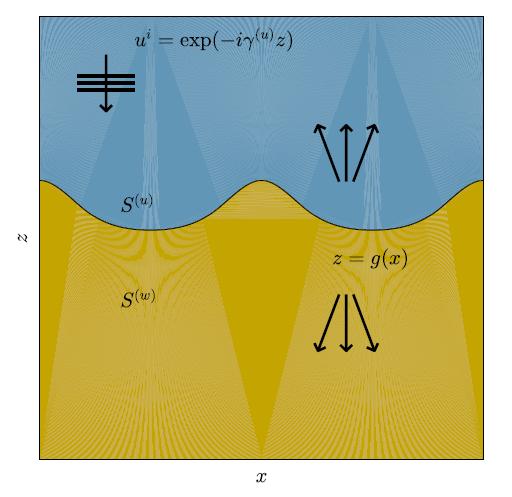
\includegraphics[width=80mm]{figures/two_layer_interface.png}
\caption{A two-layer structure with a periodic interface,
    $z=g(x)$, separating two material layers, $S^{(u)}$ and
    $S^{(w)}$, illuminated by plane--wave incidence.}
\end{center}
\end{figure}
\vspace{-22mm}
The $d$--periodic interface shape is specified by the graph of the function
$z = g(x)$, $g(x+d) = g(x)$. A dielectric (with refractive index $n^u$) 
occupies the domain above the interface
$$
S^{(u)} := \{ z > g(x) \},
$$
while a material of refractive index $n^w$ is in the lower layer
$$
S^{(w)} := \{ z < g(x) \}.
$$
The subscripts are chosen to conform to the notation of
\cite{Nicholls12,Nicholls17}.
The structure is illuminated from above by monochromatic plane--wave incident radiation
of frequency $\omega$ and wavenumber $k^u = n^u\omega/c_0=\omega/c^u$ 
($c_0$ is the speed of light) aligned with the grooves
$$
\textbf{\underline{E}}^{\text{inc}}(x,z,t) = \textbf{A} e^{-i \omega t + i \alpha x - i \gamma z},
\quad
\textbf{\underline{H}}^{\text{inc}}(x,z,t) = \textbf{B} e^{-i \omega t + i \alpha x - i \gamma z}.
$$
We consider the reduced incident fields

\begin{gather*}
\textbf{E}^{\text{inc}}(x,z) = e^{i \omega t} \textbf{\underline{E}}^{\text{inc}}(x,z,t),
\quad
\textbf{H}^{\text{inc}}(x,z) = e^{i \omega t} \textbf{\underline{H}}^{\text{inc}}(x,z,t), \\
\alpha := k^u \sin(\theta),
\quad
\gamma^u := k^u \cos(\theta),
\end{gather*}
where the time dependence $\exp(-i\omega t)$ has been factored out. 
As shown in \cite{Petit80}, the reduced electric and magnetic fields
$\{\textbf{E},\textbf{H}\}$ are $\alpha$--quasiperiodic like the incident radiation.
To close the problem we specify that the scattered radiation is ``outgoing,'' 
upward propagating in $S^{(u)}$ and downward propagating in $S^{(w)}$.

It is well known (see, e.g., $\S 1.5-\S 1.7$ and Petit \cite{Petit80}) that in this 
two--dimensional setting, the time--harmonic Maxwell equations decouple into two 
scalar Helmholtz problems which govern the Transverse Electric and 
Transverse Magnetic polarizations. We define the invariant ($y$) direction
of the scattered (electric or magnetic) fields by $\tilde{u} = \tilde{u}(x,z)$
and $\tilde{w} = \tilde{w}(x,z)$ in $S^{(u)}$ and $S^{(w)}$, respectively. The incident radiation in the upper field is defined as $\tilde{u}^i(x,z)$ (which we will also denote by $\tilde{u}^{inc}(x,z))$. In Chapters $2$ and $3$ we will factor out the phase
$\exp(i \alpha x)$ from the fields $\tilde{u}$ and $\tilde{w}$
$$
u(x,z) = e^{-i \alpha x} \tilde{u}(x,z),
\quad
w(x,z) = e^{-i \alpha x} \tilde{w}(x,z),
$$
which, we note, are $d$--periodic. This will simplify notation and, as discussed in  Chapters $2$ and $3$, also remove the phase from the relevant quantities in our governing equations.
\section{Electromagnetic Waves, Polarization, and Parameters}
\label{intro:electromagnetics_polarization}
A wave can be described as a disturbance that travels through a medium from one location to another location \cite{sanghera2011quantum}. Waves can transfer energy from one point in space to another point in space. Therefore, there are two mechanisms which specify wave properties: The disturbance which defines the wave, and the propagation of the wave. With these, we may classify waves by the following two categories:
\begin{enumerate}
    \item Longitudinal Waves: When the disturbances in a wave are parallel to the wave's propagation direction, the wave is said to be a longitudinal wave. Sound waves, for example, are longitudinal waves because the pressure change occurs parallel to the wave's propagation direction. 
    \item Transverse Waves: When the disturbances in a wave are perpendicular (at right angles) to the wave's propagation direction, the wave is called a transverse wave. Light is an example of a transverse wave, in which energy vibrates in a direction perpendicular to the wave's direction of motion. 
\end{enumerate}
Electromagnetic waves are transverse waves where both the electric and magnetic fields are perpendicular to each other and the direction of wave propagation.

\vspace{-18mm}
%
% Figure: Polarization
%
\begin{figure}[H]
\begin{center}
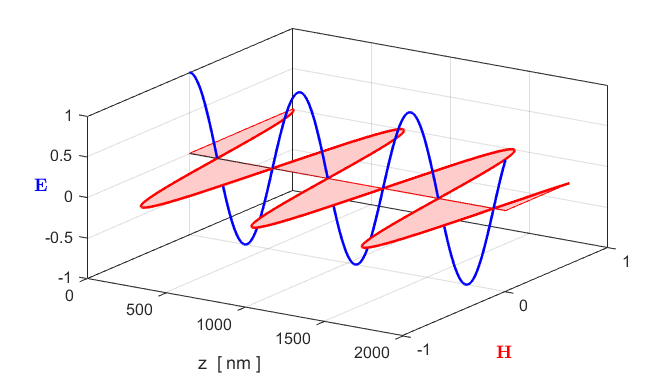
\includegraphics[scale=0.85]{figures/EM_Wave_5.png}
\vspace{0.05 mm}
\caption{A light wave is an electromagnetic wave with an electric and a magnetic component. In our scenario, the electric field $\textbf{E}$ (in blue) oscillates in the vertical direction. The magnetic field $\textbf{H}$ (in red) is at a right angle to the electric field and oscillates in the horizontal direction. Both are perpendicular to the direction of wave propagation ($\textbf{z}$).}
\end{center}
\end{figure}
\vspace{-23mm}

Electromagnetic energy is transmitted in waves 
and an electromagnetic field can propagate along various modes \cite{snyder2012optical,okamoto2021fundamentals,Jackson75}. The three most common modes are \gls{tem}, \gls{te}, and \gls{tm} where
\begin{itemize}
\item TEM Mode: In the Transverse Electric and Magnetic mode, both the electric field and the magnetic field (which, in free space, are always perpendicular to one another) are transverse (at right angles) to the direction of wave propagation (see Figure 3).
\item TE Mode: In the Transverse Electric mode, the electric field is transverse to the direction of propagation while the magnetic field is parallel to the direction of propagation.
\item TM Mode: In the Transverse Magnetic mode, the magnetic field is transverse to the direction of propagation while the electric field is parallel to the direction of propagation.
\end{itemize}
For various reasons the TM mode is of extraordinary importance (e.g., by the classical study of \gls{spr} in Raether \cite{Raether88}) and thus we concentrate our attention on the TM case in Chapters $5$ and $6.$

Throughout this thesis, we are interested in solving electromagnetic problems involving linear, homogeneous, nonmagnetic media. Our strategy, which will be discussed in detail in $\S 1.5$, is to work in the frequency domain by simplifying Maxwell's equations in matter through considering solutions where both the electric and magnetic fields are composed of time--harmonic solutions. These are solutions that have a $e^{-i\omega t}$ time--dependence for a single angular frequency $\omega$. For frequency domain problems, two key material parameters are the permittivity $\epsilon$ and permeability $\mu$. In vacuum, these two quantities are represented by $\epsilon_0$ and $\mu_0$. In addition, we are interested in representing $c$, the speed of light in vacuum, in terms of $c_0$. The index of refraction characterizes the speed of propagation of light in a medium by $n = c_0/c \ge 1$ and allows us to specify the relations
\begin{align*}
c &= \frac{c_0}{n}, &&\text{(Speed in Dielectric Material)}\\
c_0 &= \frac{1}{\sqrt{\epsilon_0\mu_0}}, &&\text{(Speed of Light in Vacuum)}\\
n &= \sqrt{\frac{\epsilon\mu}{\epsilon_0\mu_0}}, &&\text{(Refractive Index)}\\
k_0 &= \frac{\omega}{c_0}, &&\text{(Wavenumber in Vacuum)}\\
k &= nk_0, &&\text{(Wavenumber and Refractive Index)}\\
\lambda &= \frac{2\pi c_0}{\omega}. &&\text{(Wavelength)}
\end{align*}
In many cases, it is enough to specify the quantities $\omega$ and  $n$ so that the remaining dielectric parameters can be found through the permittivity and permeability of the corresponding medium. We will measure the wavelength in microns (where $1 ~\mu \text{m} = 10^{-6}~\text{m}$), as is common in many applications in engineering and photonics. An alternative would be to use nanometers where $1 ~\text{nm} = 10^{-9}~\text{m}$ or $1 ~\mu\text{m} = 10^{3}~\text{nm}$. In vacuum, we have $\epsilon_0 = 8.854187817 \times 10^{-12}~ \text{F/m}~ (\text{farards per meter}), ~\mu_0 = 1.256637061 \times 10^{-6} ~\text{H/m}~ (\text{henry per meter}),$ and the speed of light becomes $c_0 = 299,792,458~\text{m/s}$ \cite{halliday2013fundamentals}. Additionally, we will assume that every material layer is piecewise homogeneous and isotropic, so that $\epsilon$ and $\mu$ are uniform throughout all directions of the medium.
\vspace{-1.8mm}
\section{Maxwell Equations}
\label{intro:maxwell}
\vspace{-1mm}
Following \cite{Jackson75,BillinghamKing00,HOPS_Notes,Petit80,maier2007plasmonics}, we consider a region $S$ and take as a starting point Maxwell's equations of macroscopic electromagnetism in the following form:
\begin{subequations}
\begin{align}
\nabla \times \textbf{\underline{E}} &= -\frac{\partial \textbf{\underline{B}}}{\partial t}, &&\text{(Faraday's Law of Induction)}\\
\nabla \times \textbf{\underline{H}} &= \textbf{J} + \frac{\partial \textbf{\underline{D}}}{\partial t},&&\text{(Ampère's Law)}\\
\nabla\cdot \textbf{\underline{D}} &= \rho,&&\text{(Gauss's Law)}\\
\nabla\cdot \textbf{\underline{B}}&=0, &&\text{(Gauss's Law  for Magnetism)}
\end{align}
\end{subequations}
where $\textbf{J}$ is the current density and $\rho$ is the charge density. These equations link the four (time dependent) macroscopic fields
\begin{itemize}
    \item $\textbf{\underline{E}}=\textbf{\underline{E}}(x,y,z,t)$: The Electric field.
    \item $\textbf{\underline{H}}=\textbf{\underline{H}}(x,y,z,t)$: The Magnetic field.
    \item $\textbf{\underline{D}}=\textbf{\underline{D}}(x,y,z,t)$: The Electric Displacement field.
    \item $\textbf{\underline{B}}=\textbf{\underline{B}}(x,y,z,t)$: The Magnetic Induction field.
\end{itemize}
The four fields are further linked via the polarization \textbf{P} and magnetization \textbf{M} by
\begin{align*}
\textbf{\underline{D}} & = \epsilon_0\textbf{\underline{E}} + \textbf{P}, \\
\textbf{\underline{H}} & = \frac{1}{\mu_0}\textbf{\underline{B}} - \textbf{M},
\end{align*}
where $\epsilon_0$ and $\mu_0$ are the electric permittivity and magnetic permeability of vacuum. The connections between the fields depend on material properties that are defined by the quantities
\begin{itemize}
\item Polarization \textbf{P}: The electric dipole moment per unit volume.
\item  Magnetization \textbf{M}: The magnetic dipole moment per unit volume.
\end{itemize}
Limiting ourselves to linear, isotropic, homogenuous, nonmagnetic media, we define the constitutive relations
\begin{subequations}
\begin{align}
\textbf{\underline{D}}&= \epsilon_0\epsilon_r\textbf{\underline{E}},\\
\textbf{\underline{B}}&= \mu_0\mu_r\textbf{\underline{H}},
\end{align}
\end{subequations}
where $\epsilon_r$ is a dielectric constant representing the relative permittivity and $\mu_r = 1$ is relative
permeability of the nonmagnetic medium. The linear relationship between \textbf{\underline{D}} and \textbf{\underline{E}} is often implicitly defined using the dielectric susceptibility $\chi$, which describes the linear relationship between \textbf{P} and \textbf{\underline{E}} via
\bes
\textbf{P} = \epsilon_0\chi\textbf{\underline{E}}.
\ees
From here, one finds
\begin{align*}
\textbf{\underline{D}} = \epsilon_0\textbf{\underline{E}} + \textbf{P} = \epsilon_0(1+\chi)\textbf{\underline{E}},
\end{align*}
which from $(1.2\text{a})$ yields $\epsilon_r = 1+\chi.$ Substituting $(1.2)$ into $(1.1)$ produces

\begin{subequations}
\begin{align}
\nabla \times \textbf{\underline{E}} &= -\mu_0\frac{\partial \textbf{\underline{H}}}{\partial t}, \\
\nabla \times \textbf{\underline{H}} &= \textbf{J} + \epsilon_0\epsilon_r\frac{\partial \textbf{\underline{E}}}{\partial t},\\
\nabla\cdot \textbf{\underline{E}} &= \rho/(\epsilon_0\epsilon_r),\\
\nabla\cdot \textbf{\underline{H}}&=0.
\end{align}
\end{subequations}
In consideration of our particular scenario, we assume there are no free charges (requiring $\rho\equiv 0$). We model the current density with the linear relationship
$$\textbf{J}=\sigma \textbf{\underline{E}},$$
which is known as Ohm's law. The scalar $\sigma$ represents the conductivity of an isotropic material. To work in the frequency domain and obtain time-harmonic solutions of the form
\begin{equation}\textbf{\underline{E}}(x,y,z,t)=\textbf{E}(x,y,z)e^{-i\omega t},\quad \textbf{\underline{H}}(x,y,z,t)= \textbf{H}(x,y,z)e^{-i\omega t},\end{equation}
we insert $(1.4)$ into $(1.3)$ to obtain
\begin{subequations}
\begin{align}
\nabla \times \textbf{E} &= i\omega\mu_0 \textbf{H},\\
\nabla \times \textbf{H} &= -i\omega\epsilon_0\epsilon \textbf{E},\\
\nabla\cdot \textbf{E} &= 0,\\
\nabla\cdot \textbf{H}&=0,
\end{align}
\end{subequations}
where 
$$\epsilon:=\epsilon'+i\epsilon'', \quad \epsilon'=\epsilon_r, \quad \epsilon''= \sigma/(\omega\epsilon_0),$$ 
is the complex permittivity. A dielectric (or insulator) is the name given to a material for which
$$\sigma/(\omega\epsilon_0)\ll \epsilon' \implies \text{Im}(\epsilon)\approx 0,$$
and a perfect insulator is a material where $\sigma =0$ which implies $\text{Im}(\epsilon)=0$. An example is vacuum where $\epsilon =1$. A metal (or conductor) is the name given to a material which satisfies
$$\epsilon'' = \sigma/(\omega\epsilon_0)\approx \epsilon_r.$$
Examples of good conductors are copper and silver. We call a material a perfect conductor if $\sigma \to \infty$.
To arrive at the governing equations for scattered grating, we also demand that solutions are quasiperiodic

\begin{subequations}
\begin{align}
\textbf{E}(x+d_1,y+d_2,z)&=e^{i\alpha d_1 + i\beta d_2}\textbf{E}(x,y,z),\\
\textbf{H}(x+d_1,y+d_2,z)&=e^{i\alpha d_1 + i\beta d_2}\textbf{H}(x,y,z),
\end{align}
\end{subequations}
and outgoing. Then at the material interface \cite{BillinghamKing00} we have continuity of both the tangential components of the electric field and the normal components of the magnetic field. Finally, we recognize that jumps in the normal electric field and tangential magnetic field are specified by
\begin{equation}
\textbf{N}\times \textbf{E}=0, \quad \textbf{N}\times \textbf{H} = \textbf{j}_s,\quad \textbf{N}\cdot (\epsilon \textbf{E})=\rho_s, \quad \textbf{N}\cdot \textbf{H} =0,
\end{equation}
where $\textbf{N}$ is normal to the interface, $\textbf{j}_s$ represents the surface current density, and $\rho_s$ is the surface charge density. In the case that all of the permittivities and permeabilities are finite, the surface current density is zero. This allows us to enforce tangential continuity of the fields $\textbf{E}$ and $\textbf{H}$ as 
\begin{equation}
    \textbf{N}\times \textbf{E} = 0, \quad \textbf{N}\times \textbf{H} = 0.
\end{equation}
In the setting of grating structures, we choose an interface shaped by $z=g(x,y)$ and define the normal of the interface as $\textbf{N}:=(-\partial_x g, -\partial_y g,1)^T$. Therefore in a doubly layered medium our governing equations become
\vspace{-2.74mm}
\begin{subequations}
\begin{align}
\nabla \times \textbf{E}^{(u)} &= i\omega\mu_0 \textbf{H}^{(u)}, && z>g(x,y),\\
\nabla \times \textbf{H}^{(u)} &= -i\omega\epsilon_0\epsilon^{(u)} \textbf{E}^{(u)},&& z>g(x,y),\\
\nabla \times \textbf{E}^{(w)} &= i\omega\mu_0 \textbf{H}^{(w)},&& z<g(x,y),\\
\nabla \times \textbf{H}^{(w)} &= -i\omega\epsilon_0\epsilon^{(w)}  \textbf{E}^{(w)},&& z<g(x,y),\\
\textbf{N}\times \left[\textbf{E}^{(u)}-\textbf{E}^{(w)}\right]&=-\textbf{N}\times \textbf{E}^{\text{inc}},&& z=g(x,y),\\
\textbf{N}\times \left[\textbf{H}^{(u)}-\textbf{H}^{(w)}\right]&=-\textbf{N}\times \textbf{H}^{\text{inc}},&& z=g(x,y).
\end{align}
\end{subequations}
Here, $\{\textbf{E}^{(u)},\textbf{H}^{(u)}\}$ and $\{\textbf{E}^{(w)},\textbf{H}^{(w)}\}$ represent outgoing, quasiperiodic, divergence free electric and magnetic fields defined in the upper $\big(S^{(u)}=\{z > g\}\big)$ and lower $\big(S^{(w)}=$ $\{z<g\}\big)$ media. The constants  $\epsilon^{(u)}$ and $\epsilon^{(w)}$ represent the permittivities which fill the two material layers. 

To simplify future developments, we make two assumptions which allow us to focus on scalar solutions in two dimensions. Our first assumption is that the grating structure is invariant in the $y$--direction so that the interface shape becomes
\begin{align*}z=g(x).\end{align*}
This implies that $-\partial_y g=0$ and the interface normal becomes
\vspace{-0.2mm}
\begin{equation}
\textbf{N}=\begin{pmatrix}
-\partial_x g\\ 0 \\ 1
\end{pmatrix}.
\end{equation}
The second assumption is that the incident radiation is aligned with the invariant grooves of the grating structure. In this case, in \gls{te} polarization the electric field takes the form
\begin{equation}
\textbf{E}^{\text{inc}}=\textbf{E}^{\text{inc}}(x,z)=\textbf{A}e^{i\alpha x - i\gamma z},\quad \textbf{A}= 
\begin{pmatrix}
0\\ A \\ 0
\end{pmatrix},
\end{equation}
while in \gls{tm} polarization the magnetic field can be written as
\begin{equation}
\textbf{H}^{\text{inc}}=\textbf{H}^{\text{inc}}(x,z)=\textbf{B}e^{i\alpha x - i\gamma z},\quad \textbf{B}= 
\begin{pmatrix}
0\\ B \\ 0
\end{pmatrix}.
\end{equation}
\section{Tranverse Electric (TE) Polarization}
\label{intro:te_polarization}

Suppose that the electric field is transverse to the direction of propagation while the magnetic field is parallel to the direction of propagation. Then the electric field has only a transverse component and we seek solutions satisfying
\begin{equation}
\textbf{E}=\textbf{E}(x,z)=\begin{pmatrix}
0\\ \tilde{v}(x,z) \\ 0
\end{pmatrix},\quad 
\textbf{H}=\textbf{H}(x,z)=\begin{pmatrix}
H^x(x,z)\\ 0 \\ H^z(x,z)
\end{pmatrix}.
\end{equation}
In order to satisfy the time--harmonic Maxwell equations we calculate
$$\nabla \times \textbf{E}= \begin{pmatrix}
-\partial_z \tilde{v}\\ 0 \\ \partial_x \tilde{v}
\end{pmatrix},$$
which implies
$$\textbf{H} = \frac{1}{i\omega\mu_0}\nabla \times \textbf{E} =\begin{pmatrix}
-\partial_z \tilde{v}/(i\omega\mu_0)\\ 0 \\ \partial_x \tilde{v}/(i\omega\mu_0)
\end{pmatrix}.$$
Similarly,
$$\nabla \times \textbf{H}=\begin{pmatrix}
0\\ \partial_z H^x - \partial_x H^z \\ 0
\end{pmatrix},$$
so that we can reduce $(1.9\text{b})$ and $(1.9\text{d})$ from
$$-i\omega\epsilon_0\epsilon \textbf{E} = \nabla \times \textbf{H},$$
to one equation in the $y$--component
$$\text{div}\left[-\frac{1}{i\omega \mu_0}\nabla \tilde{v}\right]= - i\omega \epsilon_0\epsilon \tilde{v}.$$
As the divergence of the gradient is the Laplacian and $\mu_0$ is constant, we obtain
\begin{equation}
 0=\Delta \tilde{v} + \omega^2\mu_0\epsilon_0\epsilon \tilde{v} = \Delta \tilde{v}+\frac{\omega^2}{c_0^2}\epsilon \tilde{v}=\Delta \tilde{v}+k_0^2\epsilon \tilde{v} = \Delta \tilde{v}+k^2\tilde{v}. 
\end{equation}
The boundary conditions become
\begin{equation}
0=\textbf{N} \times \textbf{E} = \begin{pmatrix}
-\tilde{v} \\ 0 \\ -(\partial_x g)\tilde{v}
\end{pmatrix},
\end{equation}
and
\begin{equation}
0=\textbf{N} \times \textbf{H} = \begin{pmatrix}
0 \\ (\partial_x g)H^z + H^x \\ 0 
\end{pmatrix}=\frac{1}{i\omega\mu_0}\begin{pmatrix}
0 \\ (\partial_x g)\partial_x \tilde{v} - \partial_z \tilde{v} \\ 0
\end{pmatrix}.
\end{equation}
The first boundary condition $(1.15)$ shows that $\tilde{v}$ is continuous across interfaces while the second boundary condition $(1.16)$ warrants that $\partial_N \tilde{v}$ is also continuous across interfaces. This follows from the fact that $\mu_0$ is a constant equal to the permeability of vacuum in all media and is therefore constant across boundaries. As a consequence, in a doubly layered medium the TE governing equations are
\begin{subequations}
\begin{align}
\Delta \tilde{u} + (k^u)^2 \tilde{u} &=0,&& z > g(x),\\
\Delta \tilde{w} + (k^w)^2 \tilde{w} &=0,&& z < g(x),\\
\tilde{u}-\tilde{w} &= -\tilde{u}^{inc},&& z=g(x),\\
\partial_N \tilde{u}-\tau^2\partial_N \tilde{w} &= -\partial_N \tilde{u}^{inc},&& z=g(x),
\end{align}
\end{subequations}
where
\bes
\tau^2=\frac{\varepsilon^u}{\varepsilon^w}=\frac{(k^u)^2}{(k^w)^2}=\frac{(n^u)^2}{(n^w)^2},
\ees
and $\tilde{u}$ and $\tilde{w}$ are defined as outgoing, quasiperiodic solutions (in the $y$--component) of the electric field in the upper and lower layers. To clarify what is meant by solutions that are bounded, outgoing, and quasiperiodic, we will introduce an \gls{owc} in $\S 1.8$.
\section{Tranverse Magnetic (TM) Polarization}
\label{intro:tm_polarization}
If we instead assume that the magnetic field is transverse to the direction of propagation while the electric field is parallel to the direction of propagation, then the magnetic field is composed entirely of a transverse component and we seek solutions satisfying

\begin{equation}
\textbf{H}=\textbf{H}(x,z)=\begin{pmatrix}
0\\ \tilde{v}(x,z) \\ 0
\end{pmatrix},\quad 
\textbf{E}=\textbf{E}(x,z)=\begin{pmatrix}
E^x(x,z)\\ 0 \\ E^z(x,z)
\end{pmatrix}.
\end{equation}
We may once again satisfy the time--harmonic Maxwell equations by calculating
$$\nabla \times \textbf{H}= \begin{pmatrix}
-\partial_z \tilde{v}\\ 0 \\ \partial_x \tilde{v}
\end{pmatrix},$$
which implies
$$\textbf{E} = \frac{-1}{i\omega\epsilon_0\epsilon}\nabla \times \textbf{H} =\frac{1}{\epsilon}\begin{pmatrix}
\partial_z \tilde{v}/(i\omega\epsilon_0)\\ 0 \\ -\partial_x \tilde{v}/(i\omega\epsilon_0)
\end{pmatrix}.$$
Similarly to TE polarization, we find
$$\nabla \times \textbf{E}=\begin{pmatrix}
0\\ \partial_z E^x - \partial_x E^z \\ 0
\end{pmatrix},$$
and we can reduce $(1.9\text{a})$ and $(1.9\text{c})$
$$i\omega\mu_0 \textbf{H} = \nabla \times \textbf{E},$$
to one equation in the $y$--component
$$\text{div}\left[\frac{1}{i\omega \epsilon_0\epsilon}\nabla \tilde{v}\right]=  i\omega \mu_0 \tilde{v}.$$
As $\epsilon$ changes value between layers, we find
\begin{equation}
 0=\text{div}\left[\frac{1}{\epsilon}\nabla \tilde{v}\right] + \omega^2\mu_0\epsilon_0\tilde{v} = \text{div}\left[\frac{1}{\epsilon}\nabla \tilde{v}\right]+\frac{\omega^2}{c^2}\tilde{v}=\text{div}\left[\frac{1}{\epsilon}\nabla \tilde{v}\right]+k_0^2\tilde{v}. 
\end{equation}
If the layers are homogeneous then we may reduce $(1.19)$ in each layer to 
\begin{equation}
0=\Delta \tilde{v} + k^2\tilde{v}.
\end{equation}
The boundary conditions become
\begin{equation}
0=\textbf{N} \times \textbf{H} = \begin{pmatrix}
-\tilde{v} \\ 0 \\ -(\partial_x g)\tilde{v}
\end{pmatrix},
\end{equation}
and
\begin{equation}
0=\textbf{N} \times \textbf{E} = \begin{pmatrix}
0 \\ (\partial_x g)E^z + E^x \\ 0 
\end{pmatrix}=\frac{-1}{i\omega\epsilon_0}\begin{pmatrix}
0 \\ \big[(\partial_x g)\partial_x \tilde{v} - \partial_z \tilde{v}\big]/\epsilon \\ 0
\end{pmatrix}.
\end{equation}
Similarly to TE polarization, the first boundary condition $(1.21)$ shows that $\tilde{v}$ is continuous across interfaces. However, the second boundary condition $(1.22)$ mandates that $(1/\epsilon)\partial_N \tilde{v}$ is continuous across interfaces. This follows from the fact that $\epsilon_0$ is constant everywhere and $\epsilon$ is allowed to jump across layer interfaces. Therefore in a doubly layered medium the TM governing equations are
\begin{subequations}
\begin{align}
\Delta \tilde{u} + (k^u)^2 \tilde{u} &=0,&& z > g(x),\\
\Delta \tilde{w} + (k^w)^2 \tilde{w} &=0,&& z < g(x),\\
\tilde{u}-\tilde{w} &= -\tilde{u}^{inc},&& z=g(x),\\
\partial_N \tilde{u}-\tau^2\partial_N \tilde{w} &= -\partial_N \tilde{u}^{inc},&& z=g(x),
\end{align}
\end{subequations}
where, as in TE polarization, $\tilde{u}$ and $\tilde{w}$ are defined as outgoing, quasiperiodic solutions (in the $y$--component) of the magnetic field in the upper and lower layers. 


%\section{Tranverse Electromagnetic (TEM) Polarization}
\label{intro:tem_polarization}

In the most restrictive case, we assume that both the electric and magnetic fields are transverse to the direction of propagation. Then both are composed entirely of a transverse component and we seek solutions satisfying

\begin{equation}
\textbf{E}=\textbf{E}(x,z)=\begin{pmatrix}
0\\ \tilde{v}(x,z) \\ 0
\end{pmatrix},\quad 
\textbf{H}=\textbf{H}(x,z)=\begin{pmatrix}
0\\ H^y(x,z)\\ 0
\end{pmatrix}.
\end{equation}
In order to satisfy the time-harmonic Maxwell equations we calculate
$$\nabla \times \textbf{E}= \begin{pmatrix}
-\partial_z \tilde{v}\\ 0 \\ \partial_x \tilde{v}
\end{pmatrix},$$
which implies
$$\textbf{H} = \frac{1}{i\omega\mu_0}\nabla \times \textbf{E} =\begin{pmatrix}
-\partial_z \tilde{v}/(i\omega\mu_0)\\ 0 \\ \partial_x \tilde{v}/(i\omega\mu_0)
\end{pmatrix}.$$
Similarly,
$$\nabla \times \textbf{H}=\begin{pmatrix}
-\partial_z H^y\\ 0 \\ \partial_x H^y
\end{pmatrix},$$
implies
$$\textbf{E} = \frac{-1}{i\omega\varepsilon_0\varepsilon}\nabla \times \textbf{H} =\frac{1}{\varepsilon}\begin{pmatrix}
\partial_z H^y/(i\omega\varepsilon_0)\\ 0 \\ -\partial_x H^y/(i\omega\varepsilon_0)
\end{pmatrix}.$$
Upon reducing $(1.10\text{a})$ and $(1.10\text{c})$ componentwise
$$i\omega\mu_0 \textbf{H} = \nabla \times \textbf{E},$$
we find
$$\nabla \times \textbf{E}=0.$$
A similar procedure for $(1.10\text{b})$ and $(1.10\text{d})$
$$-i\omega\varepsilon_0\varepsilon \textbf{E} = \nabla \times \textbf{H},$$
gives
$$\nabla \times \textbf{H}=0.$$
The boundary conditions become
\begin{equation}
\textbf{N} \times \textbf{H} = \begin{pmatrix}
-H^y \\ 0 \\ -(\partial_x g)H^y
\end{pmatrix},
\end{equation}
and
\begin{equation}
\textbf{N} \times \textbf{E} = \begin{pmatrix}
-\tilde{v} \\ 0 \\ -(\partial_x g)\tilde{v}
\end{pmatrix}.
\end{equation}
These imply that both $\tilde{v}$ and $H^y$ are continuous across interfaces. Due to the restrictions of this mode, Maxwell's equations become
\be
\nabla \times \textbf{E} = 0, \quad \nabla \times \textbf{H} = 0, \quad \nabla \cdot \textbf{E} = 0,\quad  \nabla \cdot \textbf{H} = 0,
\ee
from which it is evident that $\textbf{E}=\textbf{H}=0$. Thus, in a doubly layered media the Transverse Electromagnetic (TEM) governing equations are
\begin{subequations}
\begin{align}
\Delta \tilde{u} + (k^u)^2 \tilde{u} &=0,&& z > g(x),\\
\Delta \tilde{w} + (k^w)^2 \tilde{w} &=0,&& z < g(x),\\
\tilde{u}-\tilde{w} &= -\tilde{u}^{inc},&& z=g(x),\\
\partial_N \tilde{u}-\partial_N \tilde{w} &= -\partial_N \tilde{u}^{inc},&& z=g(x),
\end{align}
\end{subequations}
and the only solution is the trivial solution. This implies $k^u=k^w=0$, $\tilde{u}^{inc}=0$, and the solutions $\tilde{u}$ and $\tilde{w}$ represent the trivial solution $\tilde{u}=\tilde{w}=0$. As a result, the TEM mode is rarely studied in the context of grating structures.
\section{Rayleigh Expansions}
\label{intro:rayleigh}
In order to make precise the far--field boundary conditions we desire, we study solutions of the following boundary value problem
\begin{subequations}
\begin{align}
\Delta \tilde{u} + (k^u)^2 \tilde{u} &=0,&& \text{in $S^{(u)}$},\\
\tilde{u}(x,g(x))&=\tilde{\zeta}^u(x),&& \text{at $z=g(x)$},\\
\tilde{u}(x+d,z)&=e^{i\alpha d}\tilde{u}(x,z),\\
\text{OWC}[\tilde{u}]&=0,&& z \to\infty,
\end{align}
\end{subequations}
which are outgoing, bounded, and quasiperiodic. The fourth condition $(1.24\text{d})$ mandates that solutions are both outgoing and bounded and is known as the Outgoing Wave Condition. To make these boundary conditions more precise, we first observe that for $z > a > \left| g \right|_{\infty}$ the solution to $(1.24)$ in $S^{(u)}$ is given by
\begin{align}
\tilde{u}(x,z)=\sum_{p=-\infty}^{\infty}a_pe^{i\alpha_px + i\gamma_p^u z}+ \sum_{p=-\infty}^{\infty}b_pe^{i\alpha_px - i\gamma_p^w z}.  
\end{align}
In this setting (and in many other places in this thesis), we let $p\in\mathbb Z, ~q\in\{u,w\},$ and define
\begin{align}
\alpha_p := \alpha + \left(\frac{2\pi}{d}\right)p, \quad \gamma_p^q:= \begin{cases} 
      \sqrt{(k^q)^2-\alpha_p^2}, & p\in\mathcal{U}^q, \\
      i\sqrt{\alpha_p^2-(k^q)^2}, & p\not\in\mathcal{U}^q,
   \end{cases}
\end{align}
and
\begin{align}
\mathcal{U}^q:=\{p\in\mathbb Z ~|~ \alpha_p^2 < (k^q)^2\}.
\end{align}
To enforce the requirement that our solution $(1.25)$ is outgoing and bounded, we require $b_p\equiv 0$. If $b_p\not\equiv 0$ then solutions will be inward propagating for $p\in \mathcal{U}^u$, and unbounded for $p\not \in \mathcal{U}^u$. To clarify what is meant by the Outgoing Wave Condition, we observe that for $p\in\mathcal{U}^u$, solutions are outgoing and the modes are ``propagating.'' In contrast, if $p\not\in\mathcal{U}^u$, then solutions decay exponentially and the modes are known as ``evanescent.'' Therefore the solutions of $(1.24\text{a})$ which satisfy the Outgoing Wave Condition, $(1.24\text{d})$, are
\begin{align}
\tilde{u}(x,z)=\sum_{p=-\infty}^{\infty}a_pe^{i\alpha_px + i\gamma_p^u z}.   
\end{align}
A similar argument for $z < -b < -\left| g \right|_{\infty}$ will show that solutions in the lower field which satisfy the Outgoing Wave Condition are given by
\begin{align}
\tilde{w}(x,z)=\sum_{p=-\infty}^{\infty}b_pe^{i\alpha_px - i\gamma_p^w z}.   
\end{align}
This leads to a domain decomposition of $S^{(u)}$ where we introduce an ``Artificial Boundary'' at $\{z=a\}$ and define the truncated domain 
$$S_{g,a}:= \{g(x) < z < a\}.$$
We similarly define an ``Artificial Boundary'' in the lower field, $S^{(w)}$, at $\{z=-b\}$ and define the truncated domain 
$$S_{g,-b}:= \{-b < z < g(x)\}.$$
We can now state a new boundary value problem that is equivalent to $(1.24)$ as

\begin{subequations}
\begin{align}
\Delta \tilde{u} + (k^u)^2 \tilde{u} &=0,&& \text{in $S_{g,a}$},\\
\tilde{u}(x,g(x))&=\tilde{\zeta}^u(x),&& \text{at $z=g(x)$},\\
\tilde{u}(x+d,z)&=e^{i\alpha d}\tilde{u}(x,z),\\
\Delta \tilde{v} + (k^u)^2 \tilde{v} &=0, && z>a,\\
\tilde{u}&=\tilde{v}, && \text{at $z=a$},\\
\partial_z \tilde{u} &= \partial_z \tilde{v},&& \text{at $z=a$},\\
\tilde{v}(x+d,z)&=e^{i\alpha d}\tilde{v}(x,z),\\
\text{OWC}[\tilde{v}]&=0,&& z\to\infty,
\end{align}
\end{subequations}
By the same analysis leading to $(1.28),$ solutions to $(1.30\text{d})$ are of the form
\begin{align}
\tilde{v}(x,z)=\sum_{p=-\infty}^{\infty}c_pe^{i\alpha_px + i\gamma_p^u z}.   
\end{align}
From $(1.30\text{e})$ it is clear that if we define $\psi(x):=\tilde{u}(x,a)$ and use $\tilde{v}(x,a)=\tilde{u}(x,a)$ then
$$
\tilde{v}(x,z)=\sum_{p=-\infty}^{\infty}\left(c_pe^{i\gamma_p^ua}\right)e^{i\alpha_px + i\gamma_p^u (z-a)}=\sum_{p=-\infty}^{\infty}\hat{\psi}_pe^{i\alpha_px + i\gamma_p^u (z-a)},
$$
where $\hat{\psi}_p$ are the Fourier coefficients of $\psi$. To enforce $(1.30\text{f})$ we compute
$$\partial_z \tilde{v}(x,a)=\sum_{p=-\infty}^{\infty}\left(i\gamma_p^u\right)\hat{\psi}_pe^{i\alpha_px},$$
and define the \gls{dno}
\begin{align}
\tilde{T}^u:\tilde{v}(x,a) \to \left(\partial_z \tilde{v}\right)(x,a),    
\end{align}
Equation $(1.30\text{f})$ now implies, at $z=a$,
$$0=\partial_z \tilde{u} - \partial_z \tilde{v} = \partial_z \tilde{u} - \tilde{T}^u[\tilde{v}] = \partial_z \tilde{u} - \tilde{T}^u[\tilde{u}],$$
where $$\tilde{T}^u[\psi(x)] := \sum_{p=-\infty}^{\infty}\left(i\gamma_p^u\right)\hat{\psi}_pe^{i\alpha_px}.$$ A similar calculation can be performed in the lower field. At $z=-b$ and $\psi(x):=\tilde{v}(x,-b)$ we find
$$
\tilde{v}(x,z)=\sum_{p=-\infty}^{\infty}\left(d_pe^{i\gamma_p^wb}\right)e^{i\alpha_px - i\gamma_p^w (z+b)}=\sum_{p=-\infty}^{\infty}\hat{\psi}_pe^{i\alpha_px - i\gamma_p^w (z+b)},
$$
where $\hat{\psi}_p$ are the Fourier coefficients of $\psi.$ For $z=-b$ and an equivalent representation of $(1.30)$ in the lower field, we deduce
\begin{align}
\partial_z \tilde{v}(x,-b)=\sum_{p=-\infty}^{\infty}\left(-i\gamma_p^w\right)\hat{\psi}_pe^{i\alpha_px}.
\end{align}
Hence, we may state the boundary value problem in $(1.24)$ and $(1.30)$ equivalently as
\begin{subequations}
\begin{align}
\Delta \tilde{u} + (k^u)^2 \tilde{u} &=0,&& \text{in $S_{g,a}$},\\
\tilde{u}(x,g(x))&=\tilde{\zeta}^u(x),&& \text{at $z=g(x)$},\\
\tilde{u}(x+d,z)&=e^{i\alpha d}\tilde{u}(x,z),\\
\partial_z \tilde{u} - \tilde{T}^u[\tilde{u}]&=0,&&  \text{at $z=a$.}
\end{align}
\end{subequations}
The final condition $(1.34\text{d})$ is known as a Transparent Boundary Condition at the Artificial Boundary $\{z=a\}$. A similar analysis in the lower field shows that downward propagating solutions which satisfy the Outgoing Wave Condition satisfy
$$\partial_z \tilde{w} - \tilde{T}^w[\tilde{w}]=0,\quad \text{at $z=-b$},$$
where $$\tilde{T}^w[\psi(x)] := \sum_{p=-\infty}^{\infty}\left(-i\gamma_p^w\right)\hat{\psi}_pe^{i\alpha_px},$$
and the corresponding boundary value problem becomes 
\begin{subequations}
\begin{align}
\Delta \tilde{w} + (k^w)^2 \tilde{w} &=0,&& \text{in $S_{g,-b}$},\\
\tilde{w}(x,g(x))&=\tilde{\zeta}^w(x),&& \text{at $z=g(x)$},\\
\tilde{w}(x+d,z)&=e^{i\alpha d}\tilde{w}(x,z),\\
\partial_z \tilde{w} - \tilde{T}^w[\tilde{w}]&=0,&&  \text{at $z=-b$.}
\end{align}
\end{subequations}
%\section{Separation of Variables}
\label{intro:sov}
We are interested in finding a representation of the solution $\tilde{u}$ to the boundary value problem
\begin{subequations}
\begin{align}
\Delta \tilde{u} + k^2 \tilde{u} &=0,&& \text{in $S^{(u)}$},\\
\tilde{u}(x,g(x))&=-\tilde{u}^{i}(x,g(x))=\tilde{\zeta}(x),&& \text{at $z=g(x)$},\\
\tilde{u}(x+d,z)&=e^{i\alpha d}\tilde{u}(x,z),
\end{align}
\end{subequations}
through the classical method of Separation of Variables. We split $(1.42\text{a})$ into a set of ordinary differential equations by considering 
$$\tilde{u}(x,z)=X(x)Z(z).$$
Substituting this product into the Helmholtz equation, we obtain 
$$X''Z + XZ'' + k^2XZ=0.$$
Dividing by $\tilde{u} = XZ$ and rearranging terms, we get 
\begin{align}
\frac{X''}{X}= -k^2 - \frac{Z''}{Z}.
\end{align}
Equation $(1.43)$ exhibits one Separation of Variables. The left--hand side is a function of $x$ alone, whereas the right--hand side depends only on $z$ and not on $x$. But $x$ and $z$ are independent coordinates. The equality of both sides depending on different variables means that the behavior of $x$ as an independent variable is not determined by $z$. Therefore, each side must be equal to a constant which is known as the constant of separation. We choose 
\begin{align}
  \frac{X''}{X}&=\lambda^2, \\ 
  -k^2 - \frac{Z''}{Z}&=\lambda^2.
\end{align}
Now, turning our attention to $(1.45)$, we obtain 
\begin{align}
 \frac{Z''}{Z} = -\left(\lambda^2 +k^2\right).  
\end{align}
Our goal is to solve the ODEs $(1.44)$ and $(1.46)$ through our boundary conditions. Rearranging $(1.44)$ as $X''-\lambda^2 X=0$ and solving the auxiliary equation gives
\begin{align}
\quad X_n(x)=a_ne^{\lambda x} + b_ne^{-\lambda x}.
\end{align}
Similarly, we write $(1.46)$ as $Z'' + Z\left(\lambda^2+k^2\right)=0$ and solve the auxiliary equation to find
\begin{align}
\quad Z_n(z)=c_ne^{i\sqrt{\lambda^2+k^2}z} + d_ne^{-i\sqrt{\lambda^2+k^2}z}.
\end{align}
We first analyze $(1.47)$ in combination with the boundary condition $(1.42\text{c})$ for quasiperiodic $\tilde{u}(x+d,z)=e^{i\alpha d}\tilde{u}(x,z)$. The case $d=0$ gives the trivial solution so we will assume $d\neq 0$. Now we analyze $(1.47)$ and focus on the case where $x=0$ and $d\neq 0$. The boundary condition $(1.42\text{c})$ becomes $X(d)=e^{i\alpha d}X(0)$ which, upon invoking the definition of the complex logarithm and simplifying, delivers
$$ \lambda = i\alpha+i\left(\frac{2\pi }{d}\right)p,\quad p\in\mathbb  Z, \quad d\neq 0.$$
It is clear from the left-hand side of $(1.33)$ that we may represent $\alpha_p$ by
$$ \lambda = i\alpha+i\left(\frac{2\pi }{d}\right)p=i\alpha_p,\quad p\in\mathbb  Z, \quad d\neq 0.$$
Next, we analyze the auxiliary equations when $z=0.$ The boundary condition $(1.42\text{c})$ becomes $X(x+d)=e^{i\alpha d}X(x)$ which, after some elementary computations, gives the same representation for $\lambda$. Therefore no further simplifications are necessary for $(1.47)$ and $(1.48)$. In light of this, the auxiliary equation $(1.47)$ becomes
\begin{align}
\quad X_n(x)=a_ne^{i\alpha_p x} + b_ne^{-i\alpha_p x}.
\end{align}
Inserting $\lambda=i\alpha_p$ into $(1.48)$ forms
\begin{align}
\quad Z_n(z)=c_ne^{i\sqrt{k^2-\alpha_p^2}z} + d_ne^{-i\sqrt{k^2-\alpha_p^2}z}.
\end{align}
By the right--hand side of $(1.33)$, we see that $(1.50)$ is equivalent to
\begin{align}
\quad Z_n(z)=c_ne^{i\gamma_p z} + d_ne^{-i\gamma_p z}.
\end{align}
By $(1.49),(1.51),$ and the superposition principle, the general solution is
\begin{align*}
\tilde{u}(x,z)&=\sum_{p=-\infty}^{\infty}\Big( a_pe^{i\alpha_p x} + b_pe^{-i\alpha_p x}\Big)\Big(c_pe^{i\gamma_p z} + d_pe^{-i\gamma_p z}\Big)\\&=
\sum_{p=-\infty}^{\infty}e_pe^{i\alpha_p x + i\gamma_p z} + \sum_{p=-\infty}^{\infty}f_pe^{i\alpha_p x - i\gamma_p z}.
\end{align*}
A similar calculation was made by Lord Rayleigh whose initial focus was investigating the electromagnetic problem of the diffraction of a plane wave at normal incidence \cite{rayleigh1881x,rayleigh1894theory,rayleigh1907dynamical} in a periodic structure.
%\section{Two--Layer Scattering}
\label{intro:two_layer_scattering}
Let $\tilde{u}$ be the scattered field in $S^{(u)}$ where $z>g(x)$. Then the total field is given as the sum of the scattered field and the incidence radiation
\begin{equation}
    \tilde{u}^t=\tilde{u}^i + \tilde{u}.
\end{equation}
Similarly, in $S^{(w)}$ where $z<g(x)$, there is no incidence radiation. So the total field is given by \begin{equation}
    \tilde{w}^t=\tilde{w}.
\end{equation}
The boundary conditions at the interface $z=g(x)$ are
\begin{equation}
    \tilde{u}^t = \tilde{w}^t|_{z=g}, \quad \partial_N \tilde{u}^t = \tau^2 \partial_N \tilde{w}^t|_{z=g},
\end{equation}
Therefore $(1.52)-(1.54)$ becomes
\begin{subequations}
\begin{align}
\tilde{u} + \tilde{u}^i &= \tilde{w}, &&\text{at $z=g(x)$,} \\
\partial_N \tilde{u} + \partial_N \tilde{u}^i &= \tau^2 \partial_N \tilde{w}, &&\text{at $z=g(x)$.}
\end{align}
\end{subequations}
As the incidence radiation ($\tilde{u}^i$) is an input in our system, we move it to the right--hand side. This forms the following Dirichlet and Neumann boundary conditions 
\begin{subequations}
\begin{align}
\tilde{u}-\tilde{w}&=-\tilde{u}^{i},&&\text{at $z=g(x)$,}\\
\partial_N \tilde{u}-\tau^2\partial_N \tilde{w}&=-\partial_N \tilde{u}^{i},&&\text{at $z=g(x)$,}
\end{align}
\end{subequations}
where we let $\tilde{u}^{i}:=e^{i\alpha x-i\gamma^u z}$. At the surface $z=g(x)$, we need to find the unknowns
\begin{align}
U(x)=\tilde{u}(x,z)|_{z=g(x)},\quad W(x)=\tilde{w}(x,z)|_{z=g(x)}.    
\end{align}
Our strategy is to define $\tilde{U}$ and $\tilde{W}$ so that the normal derivative is exterior pointing in the upper and lower layers. We define
\begin{align}
\tilde{U}(x):=-\partial_N \tilde{u}(x,z)|_{z=g(x)},\quad \tilde{W}(x):=\partial_N \tilde{w}(x,z)|_{z=g(x)},
\end{align}
where the operators $G$ and $J$ are
\begin{equation}G: U \to \tilde{U},\quad J: W \to \tilde{W}.\end{equation}
These operators are Dirichlet--Neumann Operators (DNOs) which connect Dirichlect and Neumann data through the pairs $\{U,\tilde{U}\}$ and $\{W,\tilde{W}\}$. Letting 
\begin{align}
\tilde{\zeta}(x):&=-\tilde{u}^{i}(x,z)|_{z=g(x)}=-e^{i\alpha x-i\gamma^u g(x)}, \\
\tilde{\psi}(x):&=-\partial_N \tilde{u}^{i}(x,z)|_{z=g(x)}=\left(i\gamma^u+i\alpha \partial_x g\right)e^{i\alpha x-i\gamma^u g(x)},
\end{align}
we see that the boundary conditions in $(1.56\text{a})-(1.56\text{b})$ may be rewritten as
\begin{align*}
U-W&=\tilde{\zeta}, &&\text{at $z=g(x)$,}\\
-\tilde{U}-\tau^2\tilde{W}&=\tilde{\psi}, &&\text{at $z=g(x)$,}
\end{align*}
or
\begin{subequations} 
\begin{align}
U-W&=\tilde{\zeta}, &&\text{at $z=g(x)$,}\\
-G[U]-\tau^2J[W]&=\tilde{\psi}, &&\text{at $z=g(x)$.} 
\end{align}
\end{subequations}
From $(1.62\text{a})$ we have $W=U-\tilde{\zeta}$. Therefore, we may write $(1.62\text{b})$ as
$$-G[U]-\tau^2J\left[U-\tilde{\zeta}\right]=\tilde{\psi},$$
which implies
\begin{equation}(G+\tau^2J)[U]=-\tilde{\psi}+\tau^2J\left[\tilde{\zeta}\right].\end{equation}
As the operators $G$ and $J$ are well--defined for sufficiently smooth $g$ (e.g., $g\in C^2$ \cite{NichollsReitich03b}) we may think of our boundary data in $(1.62\text{a})- (1.62\text{b})$ as a system of linear equations
\begin{equation}
    \bA\bV=\bR,
\end{equation}
where
\begin{equation}
 \bA=\begin{pmatrix}I & -I\\-G & -\tau^2J\end{pmatrix},\quad 
 \bV=\begin{pmatrix}U \\ W\end{pmatrix},\quad
 \bR=\begin{pmatrix}\tilde{\zeta} \\ \tilde{\psi}\end{pmatrix}.
\end{equation}
In Chapter $4$ we will show that our governing equations $(1.41)$ may be written as a linear system and discuss the motivation behind the definitions $(1.57)-(1.59)$ in terms of a Non--Overlapping \gls{ddm}. We will first remove the phase by defining $\tilde{u}(x,z):=e^{i\alpha x}u(x,z)$ and then apply two small perturbations relating to an interfacial deformation and a frequency deformation. The end result will be a linear system slightly more involved than $(1.65)$ by which interfacial data is recovered by the use of Dirichlet--Neumann Operators.

\section{Thesis Outline}
\label{intro:thesis outline}

This thesis is divided into four parts, specifically: $(1)$ Background and Introduction, $(2)$ Joint Analyticity of the Upper and Lower Fields, $(3)$ Numerical Results and Scattering, and $(4)$ Concluding Remarks and Future Research. The ``Joint Analyticity of the Upper and Lower Fields" part is contained in Chapters $2$--$4$. In Chapters $2$ and $3$, we discuss our general strategy for establishing analyticity results which are based on a special change of variables and the elliptic theory of Sobolev spaces. The concluding section of these chapters details the mechanics of our HOPS algorithm and provides example profiles where our algorithm is highly accurate and robust. Chapter $4$ combines these results to establish our main theorem (Theorem $4.6.1$) which proves the existence and uniqueness of solutions to a system of partial differential equations with respect to both interfacial and frequency deformations.

The ``Numerical Results and Scattering" part is composed of Chapters $5$ and $6$. In Chapter $5$, we describe the Method of Manufactured Solutions as a tool to demonstrate the accuracy of our HOPS algorithm. Then, in Chapter 6, we define the Reflectivity Map as a way of computing the reflected energy stored by a periodic structure. We simulate a large variety of scattering problems using a range of wavelengths and dielectric constants in both the TE and TM propagation modes. The ``Concluding Remarks" part is given in Chapter $7$ where we discuss several different possibilities for future research. Among these, the most interesting is Section $7.4$ where we analyze the necessary steps to extend our analyticality theorem from two parameters to any finite integer $M>0$.